\chapter{Shallow Water Equations}
\section{Introduction}

The shallow water equations model the height of the water front on a fluid where the mean depth is
greater than the mean amplitude. It is a hyperbolic system of partial differential equations which is
given by

\begin{align}
    \label{eq:swe1}
    \frac{\partial u}{\partial t} &= - g \frac{\partial h}{\partial x} \\
    \frac{\partial h}{\partial t} &= - H \frac{\partial u}{\partial x}
\end{align}
in one dimension and
\begin{align}
    \label{eq:swe2}
    \frac{\partial u}{\partial t} &= - g \frac{\partial h}{\partial x} + fv \\
    \frac{\partial v}{\partial t} &= -g \frac{\partial h}{\partial y} - fu\\ 
    \frac{\partial h}{\partial t} &= - H\left(\frac{\partial u}{\partial x} + \frac{\partial v}{\partial y}\right)
\end{align}
in two dimensions. The components $u, v$ are the horizontal and vertical components of the
velocity, $h$ is the difference to the fluid's mean depth $H$. Furthermore, $f$ is the Coriolis
acceleration and $g$ is the acceleration due to gravity. For more information about the
shallow water equation see \cite{Toro2024} for an in-depth treatment and \cite{Doos2022} for
an introductory exposition. The shallow water equations have various applications in modeling
geo-physical phenomena like water flow in ocean tides, breaking of waves, tsunami modeling, and roll
waves in channels. 

In this chapter, we will consider the shallow water equations in one and two dimensions for staggered and
not staggered grids for our finite difference schemes. The key idea behind staggered grids is not to
use cell average values for all quantities, but rather to measure the velocities at the
cell interfaces. This enables second order difference schemes for advection terms without
decoupling the system. They were introduced at first by \cite{Arakawa1977}.

Unless stating
otherwise, we will only consider periodic boundary conditions and thus the discretizations should
be read accordingly. Furthermore, we only consider the case where the fluid is at rest initially, i.e.
$u \equiv 0$ and respectively $v \equiv 0$. The height $h$ has a disturbance of the value $1$ at the grid's center with the same shape as the grid.

In section 2, we will present the used numerical schemes, where we will follow \cite{Doos2022}
throughout the section. The last section contains the results of our implementation.

\section{Numerical Schemes for the Shallow Water Equation}
\subsection{Schemes for the One-Dimensional Case}
At first, we determine the CFL-number for our problem. Using a Fourier Ansatz for \eqref{eq:swe1},
we arrive at the frequency equation
\begin{align*}
    \omega^2 = gHk^2
\end{align*}
and thus the phase speed is
\begin{align*}
    c = \frac{\omega}{k} = \pm \sqrt{gH}.
\end{align*}
For the one-dimensional case, we use a spatial discretization of $\Delta x= 10,000~\mathrm{m}$ with
$100$ grid points and a time step $\Delta t = 10~\mathrm{s}$. For $H = 4,000~\mathrm{m}$ and $g = 9.81
\tfrac{\mathrm{m}}{\mathrm{s}^2}$ we get the Courant number:
\begin{align*}
    \mathrm{CFL} = c \frac{\Delta t}{\Delta x} = \pm \sqrt{gH} \frac{\Delta t}{\Delta x} \approx 0.4923.
\end{align*}

We use centered finite differences for the discretization for both methods; however, the distinction
is the \emph{where} of the center and its neighboring quantities, see also Figure 7.2 in 
\cite{Doos2022}. 

In the unstaggered case, we use
\begin{align*}
    \frac{u^{n+1}_j - u^{n-1}_j}{2 \Delta t} &= -g \frac{h_{j+1}^n - h_{j-1}^n}{2 \Delta x}, \\[1em]
    \frac{h_{j}^n - h^{n-1}_{j}}{2\Delta t} &= -H \frac{u^n_{j+1} - u^n_{j-1}}{2 \Delta x}.
\end{align*}

As in the chapter before, the upper index $n$ is the time index and the lower index $j$ is the spatial
index. 


The staggered grid for the one dimensional shallow water equation measures the velocity $u$ at the
cell interfaces of our grid and not on the cell centers. Hence, the neighboring values of the height
at $u_j$ are $h_j$ and $h_{j+1}$, where we follow the convention to measure $u$ at the eastern side
of the cell. This leads to 

\begin{align*}
    \frac{u^{n+1}_j - u_j^{n-1}}{2\Delta t} &= - g \frac{h_{j+1}^n - h_j^n}{\Delta x}, \\[1em]
    \frac{h_j^{n+1} - h_{j}^{n-1}}{2\Delta t} &= -H \frac{u_j^n - u^n_{j-1}}{\Delta x}.
\end{align*}
As the authors of \cite{Doos2022} point out, the Courant number needs to be
\begin{align*}
    \mathrm{CFL} = \frac{\sqrt{gH}\, \Delta t}{\Delta x} \leq \frac{1}{2}
\end{align*}
for a stable scheme.

Since we use a leap frog scheme for the time integration, we also use a Robert-Asselin filter
to smooth out oscillations with the parameter $\gamma = 0.1$.

\subsection{Schemes for the Two-Dimensional Case}
The authors \cite{Arakawa1977} introduced staggered grids in two dimensions, and they considered several
cases, which are commonly referenced as A-grids up to E-grid. The A-grid is the unstaggered grid,
where all quantities are average values at the cell center which is given by

\begin{align}
    \label{eq:Agrid}
    \frac{\partial u_{i,j}}{\partial t} &= -g \frac{h_{i+1,j} - h_{i-1, j}}{2\, \Delta x} + f v_{i, j}, \\[1em]
    \frac{\partial v_{i,j}}{\partial t} &= -g \frac{h_{i,j+1} - h_{i, j-i}}{2\, \Delta y} + f u_{i,j}, \\[1em]
    \frac{\partial h_{i,j}}{\partial t} &= -H\left(\frac{u_{i+1,j} - u_{i-1,j}}{2\, \Delta x} + \frac{v_{i,j+1} - v_{i, j-1}}{2\, \Delta y}\right).
\end{align}
Here we use $i$ as the index for the $x$ coordinate and $j$ for the $y$ coordinate. As a time 
integrator for the unstaggered and staggered case,  we use a leapfrog scheme with a Robert-Asselin 
filter with the parameter
$\gamma = 0.1$ to smooth out the oscillations. We also experimented with other time integrators like
the Euler method, but we experienced severe instabilities. 

For the staggered C-grid we use the convention that we simulate the velocities at the 
northern and eastern sides of the cell. This leads to 

\begin{align}
    \label{eq:Cgrid}
    \frac{\partial u_{i,j}}{\partial t} &= -g \frac{h_{i+1,j }- h_{i,j}}{\Delta x} - \frac{f}{4}
    \left(\,v_{i,j} + v_{i+1,j} + v_{i+1, j-1} + v_{i,j-1}\, \right), \\[1em]
    \frac{\partial v_{i,j}}{\partial t} &= -g \frac{h_{i,j+1} - h_{i,j}}{\Delta y} - \frac{f}{4}
    \left(\,u_{i,j} + u_{i+1,j} + u_{i+1, j-1} + u_{i,j-1}\, \right), \\[1em]
    \frac{\partial h_{i,j}}{\partial t} &= -H\left(\, \frac{u_{i,j} - u_{i-1, j}}{\Delta x} + \frac{v_{i,j} - v_{i, j-1}}{\Delta y}\, \right).
\end{align}


Since there is no direct value for the velocities at the same point, we take the average around 
each point to approximate it.

The authors of \cite{Doos2022} also perform a von Neumann stability analysis and conclude that
\begin{align*}
    \mathrm{CFL} = \frac{\sqrt{gH}\, \Delta t}{\Delta x} \leq \frac{1}{\sqrt{8}} \approx 0.3535
\end{align*}
as a necessary condition for stability.


We implemented the Arakawa A-grid and C-grid in \texttt{Julia} and generate the plots using the
package \texttt{Plots}. It can be reviewed under \url{https://github.com/NiclRich/NumericalMeteorology}.


\section{Results and Conclusion}

As expected from the literature, we see better results for the staggered grids in terms of 
stability. Unlike the advection equation, we need smaller time steps as these are only conditionally stable.
Furthermore, we see smoother results, see also figure~\cref{fig:1dswe} for the one-dimensional 
shallow water equation. The figure~\cref{fig:2dswe} shows the two-dimensional shallow water
equation using the Arakawa C-grid with Coriolis $f = 10^{-4}$ and no Coriolis force. We see that the
Arakawa-C-grid captures also the Coriolis force and it is used for the conservative schemes, see
\cite{Doos2022} for more information. We conclude that the C-grid is preferable to the A-grid from a
mathematical perspective. However, different fields of science have different needs and thus they focus 
on capturing certain physical effects. Since the author's knowledge on physics is limited, we omit
the physical interpretation.

\begin{figure}[h]
    \centering

    % Row 1
    \begin{subfigure}[b]{0.3\textwidth}
        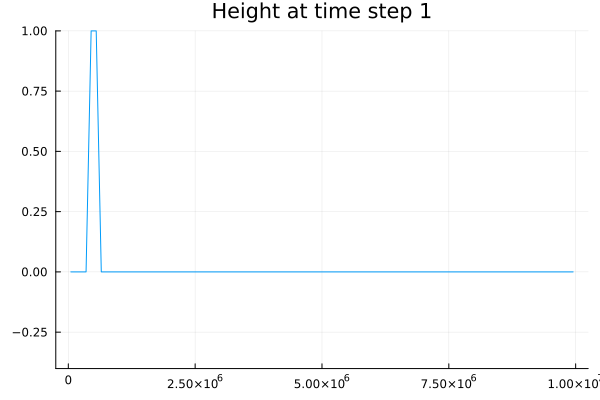
\includegraphics[width=\textwidth]{./images/height-swe1d-unstaggered-grid-1.png}
        \caption{Numerical solution of the shallow water equation at timestep 1 with unstaggered grids.}
        \label{fig:unstaggered1}
    \end{subfigure}
    \hfill
    \begin{subfigure}[b]{0.3\textwidth}
        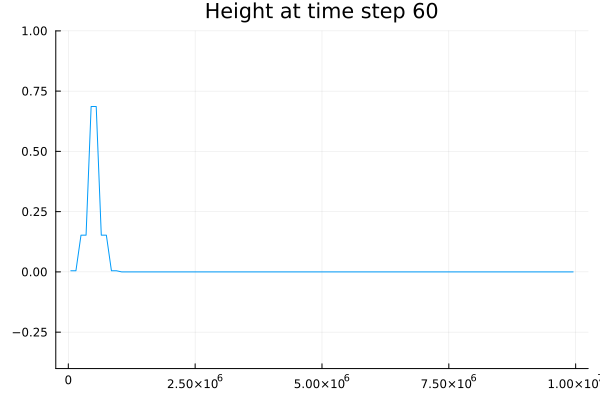
\includegraphics[width=\textwidth]{./images/height-swe1d-unstaggered-grid-60.png}
        \caption{Numerical solution of the shallow water equation at timestep 60 with unstaggered grids.}
        \label{fig:unstaggered60}
    \end{subfigure}
    \hfill
    \begin{subfigure}[b]{0.3\textwidth}
        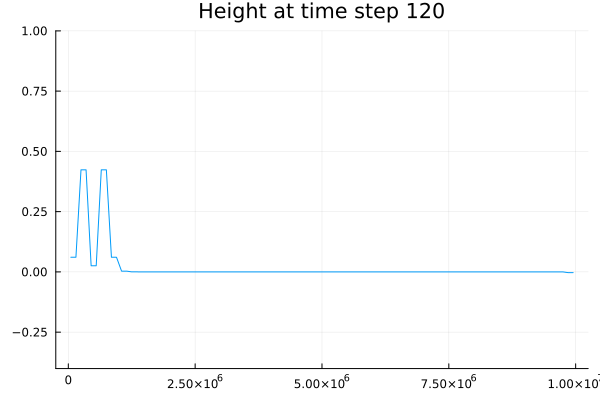
\includegraphics[width=\textwidth]{./images/height-swe1d-unstaggered-grid-120.png}
        \caption{Numerical solution of the shallow water equation at timestep 120 with unstaggered grids.}
        \label{fig:unstaggered120}
    \end{subfigure}

    \vspace{0.5cm} % Space between rows

    % Row 2
    \begin{subfigure}[b]{0.3\textwidth}
        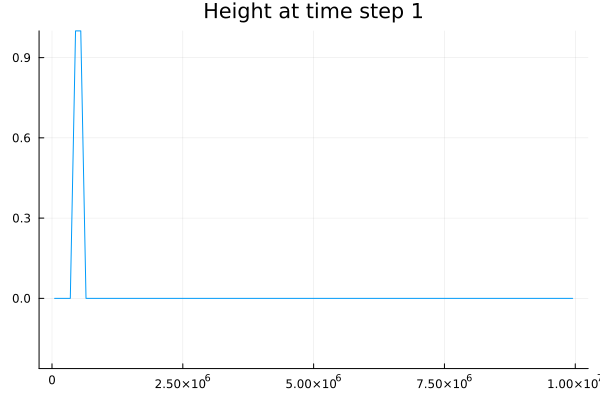
\includegraphics[width=\textwidth]{./images/height-swe1d-staggered-grid-1.png}
        \caption{Numerical solution of the shallow water equation at timestep 1 with staggered grids.}
        \label{fig:staggered1}
    \end{subfigure}
    \hfill
    \begin{subfigure}[b]{0.3\textwidth}
        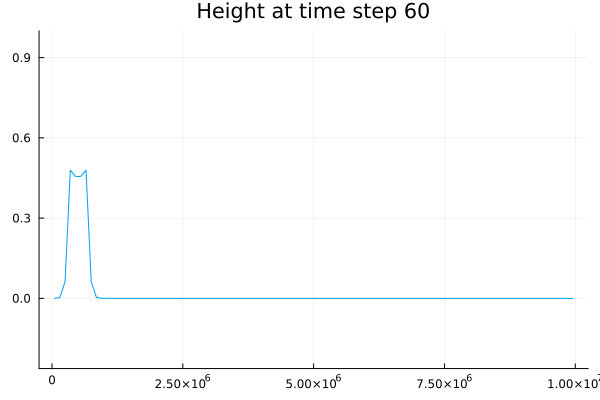
\includegraphics[width=\textwidth]{./images/height-swe1d-staggered-grid-60.png}
        \caption{Numerical solution of the shallow water equation at timestep 60 with staggered grids.}
        \label{fig:staggered60}
    \end{subfigure}
    \hfill
    \begin{subfigure}[b]{0.3\textwidth}
        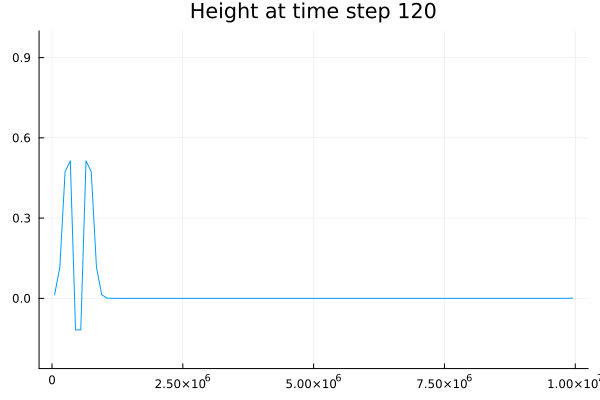
\includegraphics[width=\textwidth]{./images/height-swe1d-staggered-grid-120.png}
        \caption{Numerical solution of the shallow water equation at timestep 120 with staggered grids.}
        \label{fig:staggered120}
    \end{subfigure}

    \caption{Comparison of staggered and unstaggered grids for the one-dimensional shallow water equation.}
    \label{fig:1dswe}
\end{figure}


\begin{figure}[h]
    \centering

    % Row 1
    \begin{subfigure}[b]{0.3\textwidth}
        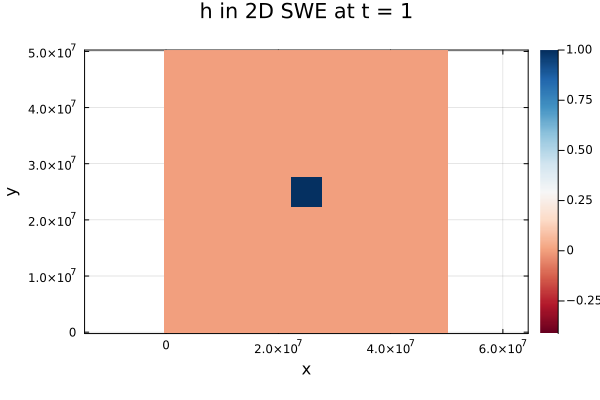
\includegraphics[width=\textwidth]{./images/swe2d-coriolis-1.png}
        \caption{Numerical solution of the shallow water equation at timestep 1 with the Arakawa C-grid.}
        \label{fig:coriolis1}
    \end{subfigure}
    \hfill
    \begin{subfigure}[b]{0.3\textwidth}
        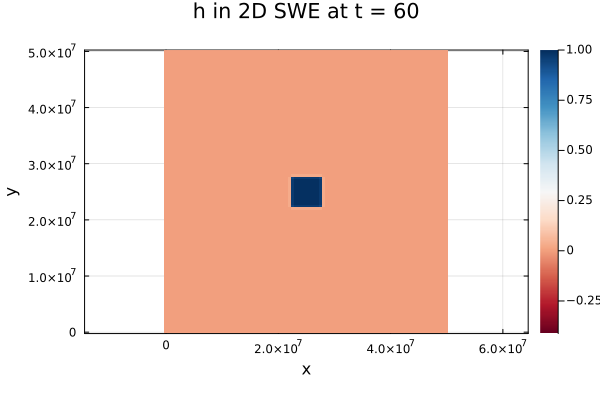
\includegraphics[width=\textwidth]{./images/swe2d-coriolis-60.png}
        \caption{Numerical solution of the shallow water equation at timestep 60 with the Arakawa C-grid.}
        \label{fig:coriolis60}
    \end{subfigure}
    \hfill
    \begin{subfigure}[b]{0.3\textwidth}
        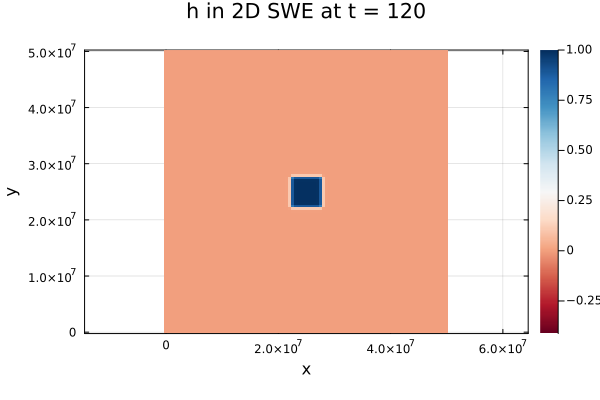
\includegraphics[width=\textwidth]{./images/swe2d-coriolis-120.png}
        \caption{Numerical solution of the shallow water equation at timestep 120 with the Arakawa C-grid.}
        \label{fig:coriolis120}
    \end{subfigure}
    \vspace{0.5cm} % Space between rows

    % Row 2
    \begin{subfigure}[b]{0.3\textwidth}
        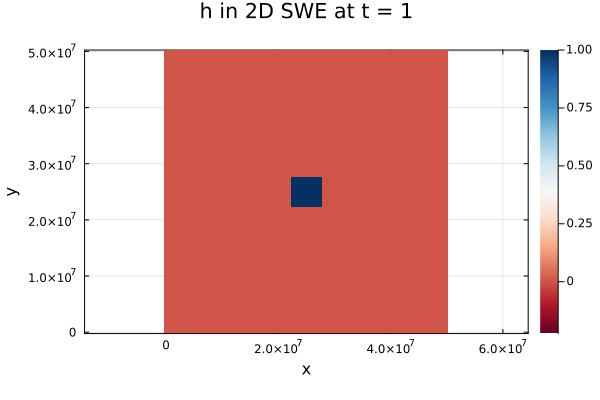
\includegraphics[width=\textwidth]{./images/swe2d-no-coriolis-1.png}
        \caption{Numerical solution of the shallow water equation at timestep 1 with the Arakawa C-grid.}
        \label{fig:nocoriolis1}
    \end{subfigure}
    \hfill
    \begin{subfigure}[b]{0.3\textwidth}
        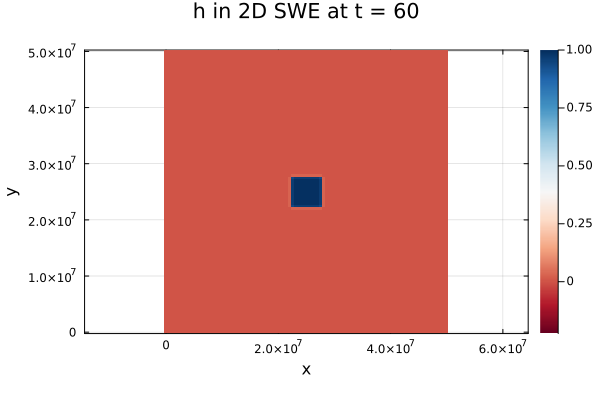
\includegraphics[width=\textwidth]{./images/swe2d-no-coriolis-60.png}
        \caption{Numerical solution of the shallow water equation at timestep 60 with the Arakawa C-grid.}
        \label{fig:nocoriolis60}
    \end{subfigure}
    \hfill
    \begin{subfigure}[b]{0.3\textwidth}
        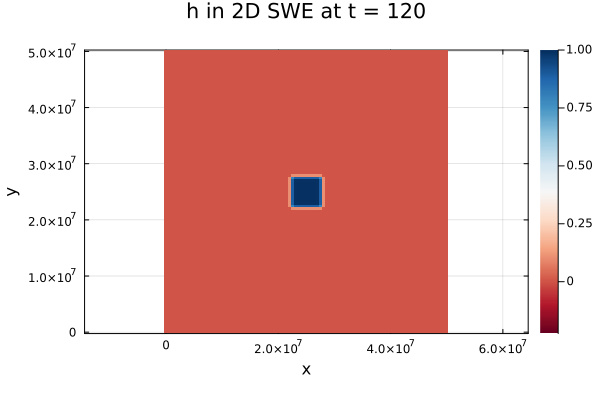
\includegraphics[width=\textwidth]{./images/swe2d-no-coriolis-120.png}
        \caption{Numerical solution of the shallow water equation at timestep 120 with the Arakawa C-grid.}
        \label{fig:nocoriolis120}
    \end{subfigure}
    \label{fig:2dswe}
\end{figure}